\chapter{المحاليل والذوبانية}\label{ch:g6:solutions-and-solubility}

تُفتح قارورة ماء فوّار: يُسمع فحيح، ويندفع سيل من الفقاعات الدقيقة يصعد
من لا مكان. كان الماء يبدو رائقًا تمامًا قبل ثانية، ومع ذلك كان فيه غاز
ذائب طوال الوقت. الأجسام الصلبة تذوب، والسوائل تذوب، والغازات تذوب
أيضًا --- لكن لا بلا حد أبدًا. يسمّي هذا الفصل أجزاء \omterm{def:g2:mixing-and-dissolving:dissolve}{المحلول}، ويقيس
مقدار ما يستطيع سائل أن يحمله من مادة ما.

\begin{recall}
الجسم الصلب الذي \omterm{def:g2:mixing-and-dissolving:dissolve}{يذوب} في الماء يختفي عن العين ويترك السائل رائقًا؛
والسائل الرائق \omterm{def:g2:mixing-and-dissolving:dissolve}{محلول}، وما ذاب فيه لا يزال موجودًا
(\cref{ch:g2:mixing-and-dissolving}). \omterm{def:g2:mixing-and-dissolving:dissolve}{والمحلول} \omterm{def:g6:pure-substances-and-mixtures:homogeneous}{خليط متجانس} من أنواع
كيميائية (\cref{ch:g6:pure-substances-and-mixtures}). \omterm{def:g3:separating-mixtures:evaporate}{وتبخير} الماء
يعيد الجسم الصلب الذائب (\cref{ch:g3:separating-mixtures}).
\end{recall}

\begin{omfigure}
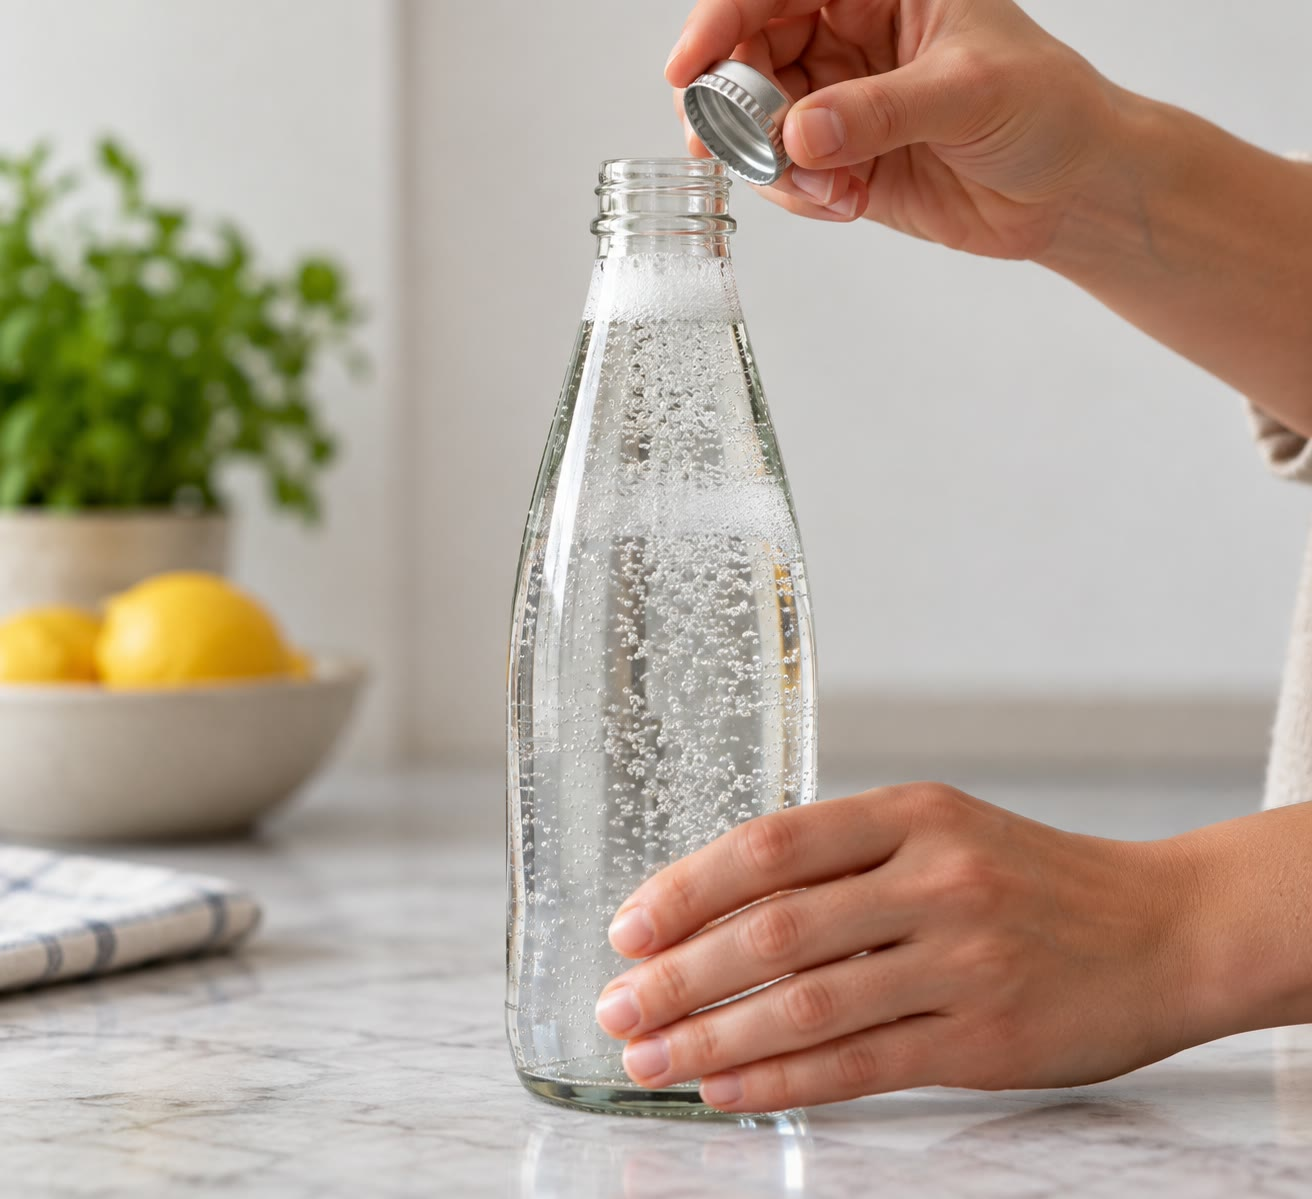
\includegraphics[width=0.5\linewidth]{images/book1/ai/g6-fizzy-water.jpg}

{\small فتح قارورة ماء فوّار: يخرج الغاز الذائب
فقاعاتٍ.}
\end{omfigure}

\section{المذاب والمذيب}

\begin{definition}[المذاب، والمذيب، والمحلول المائي]\label{def:g6:solutions-and-solubility:solute}
في \omterm{def:g2:mixing-and-dissolving:dissolve}{المحلول} تسمى المادة التي تذوب \emph{المذاب}\index{مذاب}، ويسمى
السائل الذي تذوب فيه \emph{المذيب}\index{مذيب}. وإذا كان المذيب هو
الماء سُمي \omterm{def:g2:mixing-and-dissolving:dissolve}{المحلول} \emph{محلولًا مائيًا}\index{محلول مائي}.
\end{definition}

\begin{example}[مذيبات غير الماء]\label{ex:g6:solutions-and-solubility:solvents}
الماء أشيع المذيبات، لكنه ليس الوحيد. فطلاء الأظافر لا \omterm{def:g2:mixing-and-dissolving:dissolve}{يذوب} في الماء؛
بل \omterm{def:g2:mixing-and-dissolving:dissolve}{يذوب} في البروبانون (الأسيتون)، وهو \omterm{def:g6:solutions-and-solubility:solute}{مذيب} مزيل طلاء الأظافر. والشحوم
وألوان الزيت تذوب في التربنتين المعدني. وكثير من الأدوية يُذاب في
الإيثانول. وقد يكون \omterm{def:g2:mixing-and-dissolving:dissolve}{للمحلول} عدة مذابات: فماء البحر يحوي ملحًا ذائبًا
ومواد كثيرة أخرى.
\end{example}

\begin{safety}{\ghs{GHS02}\ghs{GHS07}}
% ledger: ghs:acetone
البروبانون (الأسيتون): سائل وبخار شديدا القابلية للاشتعال (GHS02)؛ وهو
يهيّج العينين وقد يسبب بخاره النعاس أو الدوار (GHS07). ويُستعمل في
غرفة جيدة التهوية، بعيدًا عن أي لهب.
\end{safety}

\begin{proposition}[الكتل تُجمع]\label{prop:g6:solutions-and-solubility:mass}
كتلة \omterm{def:g2:mixing-and-dissolving:dissolve}{المحلول} تساوي كتلة \omterm{def:g6:solutions-and-solubility:solute}{المذيب} مضافًا إليها كتلة \omterm{def:g6:solutions-and-solubility:solute}{المذاب} الذائب: فلا يضيع
شيء حين \omterm{def:g2:mixing-and-dissolving:dissolve}{يذوب} جسم صلب، وإن لم يعد يُرى.
\end{proposition}

\begin{omfigure}
\begin{tikzpicture}[font=\small, scale=1.15]
  \pic[transform shape] at (0,0) {balance};
  \pic[transform shape] at (0,0.8) {beaker={0.5}{omWater!80}};
  \node[anchor=north, align=center] at (0,-0.1) {\foreignlanguage{arabic}{\qty{100}{g} من الماء}};
  \node at (1.85,1.3) {$+$};
  \pic[transform shape] at (3.5,0) {balance};
  \fill[white, draw=black!45] (3.0,0.8) rectangle (4.0,0.9);
  \fill[white, draw=black!45] (3.15,0.9) -- (3.85,0.9) -- (3.5,1.2) -- cycle;
  \node[anchor=north, align=center] at (3.5,-0.1) {\foreignlanguage{arabic}{\qty{10}{g} من السكر}};
  \draw[->, thick, omProp] (4.9,1.2) -- (6.0,1.2) node[midway, above, text=black]
    {التحريك};
  \pic[transform shape] at (7.4,0) {balance};
  \pic[transform shape] at (7.4,0.8) {beaker={0.52}{omWater!80}};
  \node[anchor=north, align=center] at (7.4,-0.1) {\foreignlanguage{arabic}{\qty{110}{g} من الماء المحلّى}};
\end{tikzpicture}

{\small إذابة \qty{10}{g} من السكر في \qty{100}{g} من الماء تعطي
\qty{110}{g} من \omterm{def:g2:mixing-and-dissolving:dissolve}{المحلول} (دون حساب كتلة الكأس).}
\end{omfigure}

\section{الإشباع والذوبانية}

\begin{definition}[المحلول المشبع]\label{def:g6:solutions-and-solubility:saturated}
يكون \omterm{def:g2:mixing-and-dissolving:dissolve}{المحلول} \emph{محلولًا مشبعًا}\index{محلول مشبع} إذا لم يعد قادرًا على
إذابة مزيد من مذابه: فكل \omterm{def:g6:solutions-and-solubility:solute}{مذاب} يُضاف إليه يبقى في القاع دون أن \omterm{def:g2:mixing-and-dissolving:dissolve}{يذوب}، مهما
طال التحريك.
\end{definition}

\begin{definition}[الذوبانية]\label{def:g6:solutions-and-solubility:solubility}
\emph{ذوبانية}\index{ذوبانية} \omterm{def:g6:solutions-and-solubility:solute}{مذاب} في \omterm{def:g6:solutions-and-solubility:solute}{مذيب} هي أكبر كتلة من \omterm{def:g6:solutions-and-solubility:solute}{المذاب} يستطيع
مقدار معيّن من \omterm{def:g6:solutions-and-solubility:solute}{المذيب} أن يذيبها، عند درجة حرارة معيّنة. وتُعطى ذوبانية
جسم صلب في الماء غالبًا بالغرام في اللتر (أو في الكيلوغرام) من
الماء.
\end{definition}

\begin{proposition}[ذوبانيات بعض المواد في الماء]\label{prop:g6:solutions-and-solubility:values}
% ledger: sol:NaCl, sol:sucrose, sol:CO2, sol:O2 (O2: 31 mL/L, 31/24.0 x 32 = 0.041 g/L at 20 C)
تختلف الذوبانيات المقيسة في الماء اختلافًا هائلًا:
\begin{center}
\small
\begin{tabular}{lll}
\hline
\omterm{def:g6:solutions-and-solubility:solute}{المذاب} & \omterm{def:g6:solutions-and-solubility:solubility}{الذوبانية} في الماء & الشروط \\
\hline
السكر (السكروز) & نحو \qty{2000}{g} في لتر الماء & درجة حرارة الغرفة \\
الملح (كلوريد الصوديوم) & \qty{360}{g} في كيلوغرام الماء & \qty{25}{\celsius} \\
ثنائي أكسيد الكربون & نحو \qty{1.5}{g} في اللتر & \qty{25}{\celsius}، تحت الغاز \\
الأكسجين & نحو \qty{0.04}{g} في اللتر & \qty{20}{\celsius}، تحت الغاز \\
الرمل، الطباشير & تكاد تنعدم & --- \\
\hline
\end{tabular}
\end{center}
يستطيع لتر من الماء أن يذيب من السكر أكثر من كتلته، لكنه لا يذيب
حتى نصف غرام من الأكسجين.
\end{proposition}

\begin{method}[هل يذوب كله؟]\label{met:g6:solutions-and-solubility:will-it}
لتعرف هل تذوب كتلة $m$ من \omterm{def:g6:solutions-and-solubility:solute}{مذاب} كلها في حجم معيّن من
الماء:
\begin{enumerate}
  \item جد \omterm{def:g6:solutions-and-solubility:solubility}{ذوبانية} \omterm{def:g6:solutions-and-solubility:solute}{المذاب} (بالغرام في لتر الماء)؛
  \item احسب أكبر كتلة يستطيع هذا الحجم من الماء أن يذيبها؛
  \item قارنها بالكتلة $m$: إذا كانت $m$ أصغر ذاب كل شيء؛ وإذا كانت $m$
        أكبر كان \omterm{def:g2:mixing-and-dissolving:dissolve}{المحلول} مشبعًا وبقي الباقي في
        القاع.
\end{enumerate}
\end{method}

\begin{example}[ملح في كأس]\label{ex:g6:solutions-and-solubility:glass}
% ledger: sol:NaCl
هل يمكن أن تذوب \qty{50}{g} من الملح في \qty{200}{mL} من الماء (نحو
\qty{200}{g})؟ كيلوغرام من الماء يذيب على الأكثر \qty{360}{g} من
الملح، إذن \qty{200}{g} من الماء تذيب على الأكثر $360 \times
\frac{200}{1000} = \qty{72}{g}$. وبما أن $50 < 72$ فإن الملح كله
\omterm{def:g2:mixing-and-dissolving:dissolve}{يذوب}.
\end{example}

\begin{omfigure}
\begin{tikzpicture}[font=\small, scale=1.15]
  \pic[transform shape] at (0,0) {beaker={0.6}{omWater!80}};
  \node[anchor=north, align=center] at (0,-0.15) {قليل من الملح:\\ ذاب كله};
  \pic[transform shape] at (3.2,0) {beaker={0.6}{omWater!80}};
  \node[anchor=north, align=center] at (3.2,-0.15) {ملح أكثر:\\ مشبع بالكاد};
  \pic[transform shape] at (6.4,0) {beaker={0.6}{omWater!80}};
  \fill[black!12, draw=black!50] (5.7,0) -- (7.1,0) -- (6.9,0.2) -- (5.9,0.2) -- cycle;
  \foreach \x in {5.85,6.05,6.25,6.45,6.65,6.85} \fill[black!45] (\x,0.09) circle (0.03);
  \node[anchor=north, align=center] at (6.4,-0.15) {ملح زائد:\\ يبقى الباقي غير ذائب};
\end{tikzpicture}

{\small نضيف مزيدًا من الملح إلى الماء نفسه. وما إن يصير \omterm{def:g2:mixing-and-dissolving:dissolve}{المحلول}
مشبعًا حتى يبقى الملح الزائد في القاع.}
\end{omfigure}

\begin{inthelab}[إشباع الماء المالح]
يضيف المعلم الملح إلى \qty{100}{mL} من الماء ملعقة بعد ملعقة، ويحرّك
جيدًا بعد كل واحدة. تختفي الملاعق الأولى؛ ثم تأتي ملعقة لا تذوب كلها
فتبقى حبيبات بيضاء في القاع: لقد صار \omterm{def:g2:mixing-and-dissolving:dissolve}{المحلول} مشبعًا. ويبيّن وزن الملح
المستعمل أن نحو \qty{36}{g} منه قد ذابت.
\end{inthelab}

\section{السوائل القابلة للامتزاج وغير القابلة للامتزاج}

\begin{definition}[السوائل القابلة للامتزاج وغير القابلة للامتزاج]\label{def:g6:solutions-and-solubility:miscible}
يكون السائلان \emph{قابلين للامتزاج}\index{قابل للامتزاج} إذا أعطى خلطهما
سائلًا واحدًا متجانسًا. ويكونان \emph{غير قابلين
للامتزاج}\index{غير قابل للامتزاج} إذا انفصلا في طبقتين، الأخف منهما في
الأعلى.
\end{definition}

\begin{example}[الماء مع الإيثانول، والماء مع الزيت]\label{ex:g6:solutions-and-solubility:liquids}
الماء والإيثانول قابلان للامتزاج: إذا رُجّا معًا أعطيا سائلًا واحدًا رائقًا.
أما الماء والزيت \omterm{def:g6:solutions-and-solubility:miscible}{فغير قابلين للامتزاج}: فمهما اشتد رجّهما يعود الزيت إلى
الأعلى ويطفو فوق الماء في طبقة منفصلة. وفي مرطبان صلصة السلطة يطفو الزيت
فوق الخل، والخل في معظمه ماء.
\end{example}

\begin{omfigure}
\begin{tikzpicture}[font=\small, scale=1.3]
  \pic[transform shape] at (0,0) {testtube={0.6}{omWater!80}};
  \node[anchor=north, align=center] at (0,-0.15) {ماء + إيثانول:\\ طبقة واحدة};
  \pic[transform shape] at (3,0) {testtube={0.65}{yellow!55!orange!60}};
  \begin{scope}
    \clip (2.75,3) -- (2.75,0.25) arc[start angle=180, end angle=360, radius=0.25]
      -- (3.25,3) -- cycle;
    \fill[omWater!80] (2.7,0) rectangle (3.3,1.1);
  \end{scope}
  \draw[omGlass, line width=0.7pt] (2.75,3) -- (2.75,0.25) arc[start angle=180,
    end angle=360, radius=0.25] -- (3.25,3);
  \draw[<-, omProp, thick] (3.3,1.55) -- (4.1,1.75) node[right, text=black] {زيت};
  \draw[<-, omProp, thick] (3.3,0.6) -- (4.1,0.6) node[right, text=black] {ماء};
  \node[anchor=north, align=center] at (3,-0.15) {ماء + زيت:\\ طبقتان};
\end{tikzpicture}

{\small السوائل القابلة للامتزاج تعطي طبقة واحدة؛ وغير القابلة للامتزاج تعطي طبقتين.}
\end{omfigure}

\begin{omfigure}
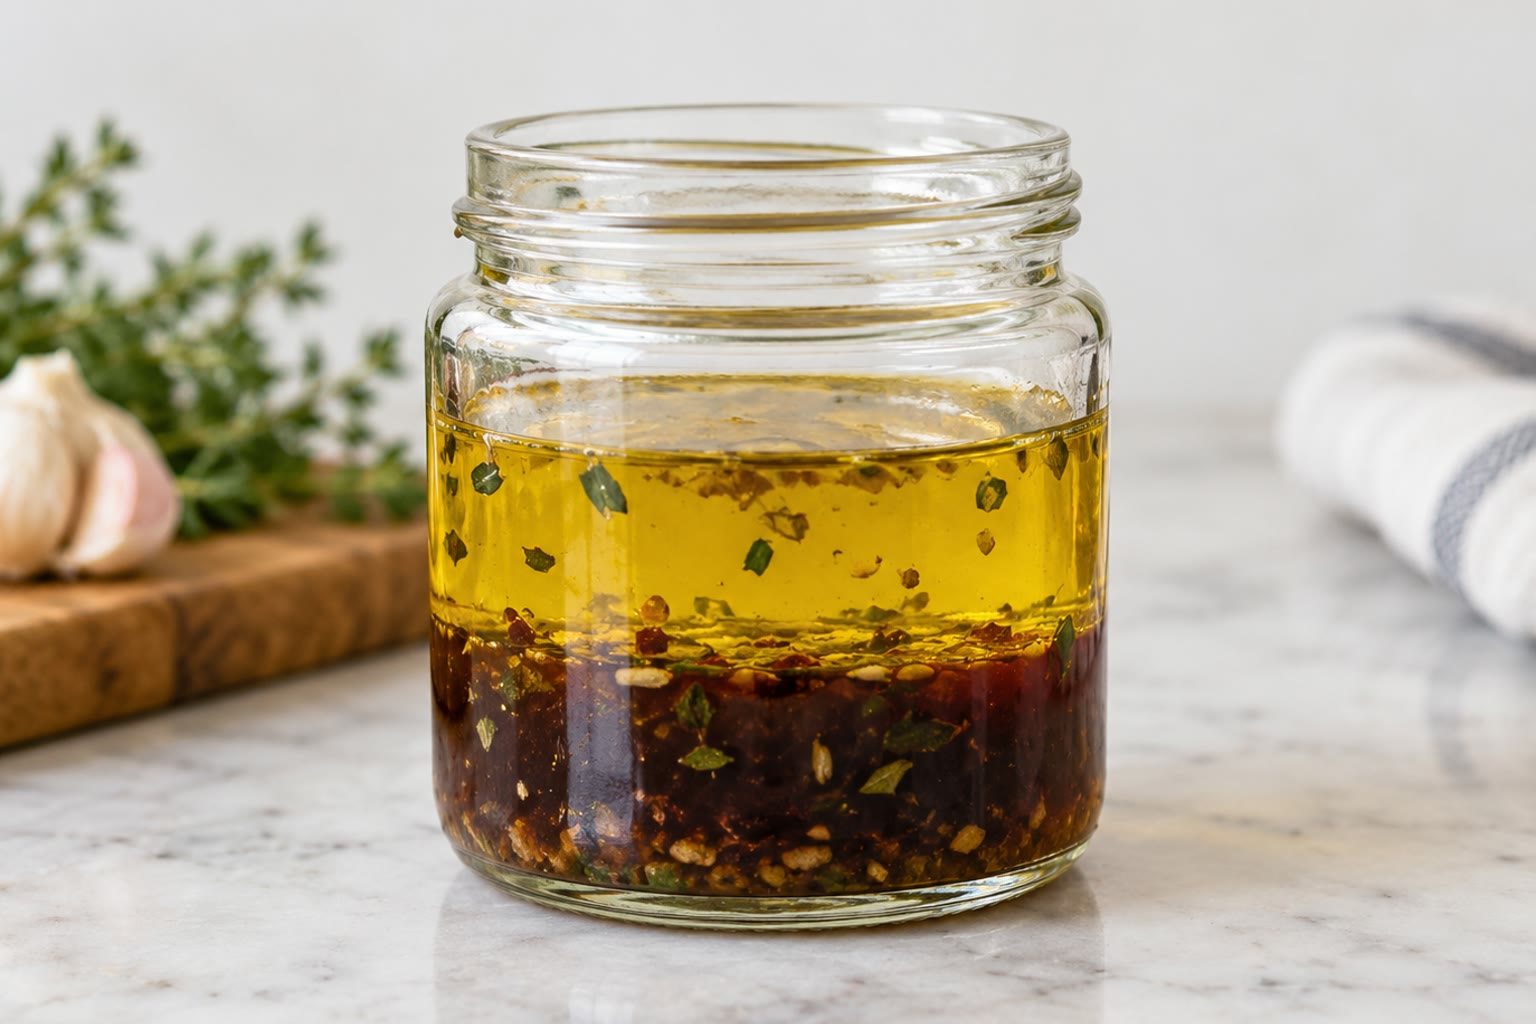
\includegraphics[width=0.45\linewidth]{images/book1/ai/g6-vinaigrette.jpg}

{\small صلصة السلطة: الزيت والخل \omterm{def:g6:solutions-and-solubility:miscible}{غير قابلين للامتزاج}.}
\end{omfigure}

\section{الغازات تذوب أيضًا}

\begin{proposition}[الغازات الذائبة]\label{prop:g6:solutions-and-solubility:gases}
تذوب الغازات في الماء، قليلًا. فالمشروبات الغازية تُصنع بإذابة ثنائي أكسيد
الكربون فيها تحت الضغط في قارورة مغلقة؛ وحين تُفتح القارورة يخرج جزء من
الغاز فقاعاتٍ. والماء الملامس \omterm{def:g4:air-a-mixture-of-gases:air}{للهواء} يحوي بعض الأكسجين الذائب، الذي
تأخذه الأسماك بخياشيمها. والغاز \omterm{def:g2:mixing-and-dissolving:dissolve}{يذوب} في الماء الدافئ أقل مما \omterm{def:g2:mixing-and-dissolving:dissolve}{يذوب} في
الماء البارد: فالمشروب الغازي الدافئ يفقد فورانه أسرع.
\end{proposition}

\begin{example}[المحيطات وثنائي أكسيد الكربون]\label{ex:g6:solutions-and-solubility:oceans}
تلامس المحيطات \omterm{def:g4:air-a-mixture-of-gases:air}{الهواء} على ثلثي سطح الأرض. \omterm{def:g2:mixing-and-dissolving:dissolve}{فيذوب} فيها ثنائي أكسيد الكربون
الذي في \omterm{def:g4:air-a-mixture-of-gases:air}{الهواء}، وبذلك تمتص المحيطات جزءًا من ثنائي أكسيد الكربون الذي
يطلقه الناس في \omterm{def:g4:air-a-mixture-of-gases:air}{الهواء}.
\end{example}

\begin{omfigure}
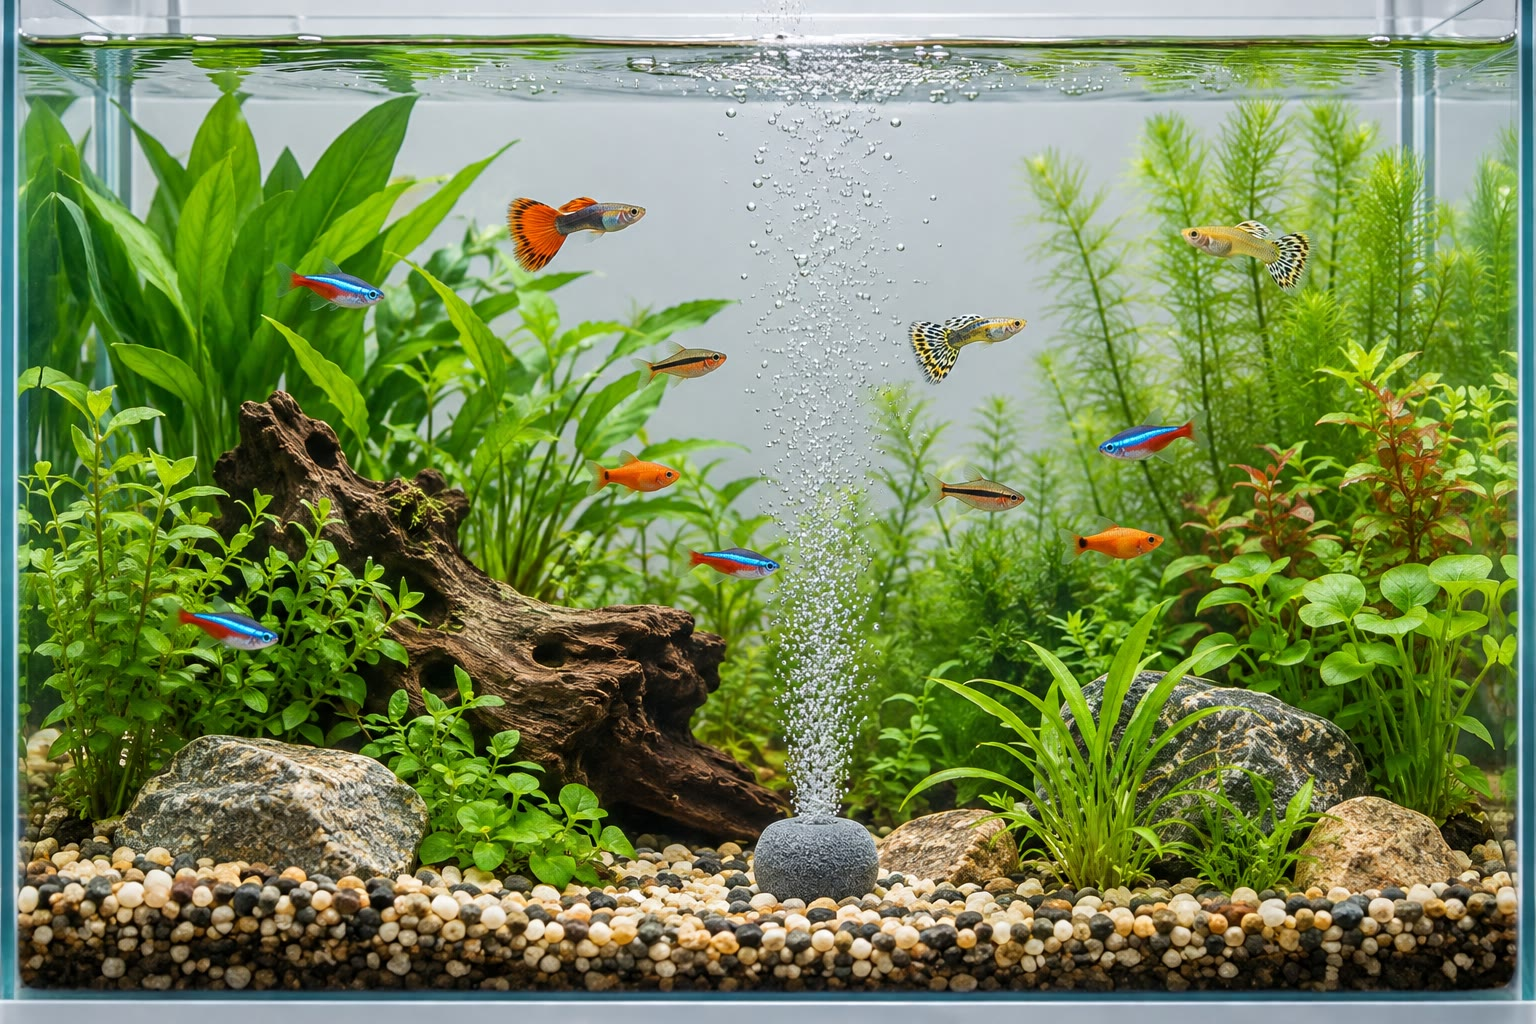
\includegraphics[width=0.5\linewidth]{images/book1/ai/g6-fish-tank.jpg}

{\small حوض أسماك: فقاعات \omterm{def:g4:air-a-mixture-of-gases:air}{الهواء} تمدّ الماء بالأكسجين الذائب
الذي تحتاج إليه الأسماك.}
\end{omfigure}

\section{تمارين}

\begin{exercise}[$\star$]\label{exo:g6:solutions-and-solubility:1}
في الماء المحلّى، سمِّ \omterm{def:g6:solutions-and-solubility:solute}{المذاب} \omterm{def:g6:solutions-and-solubility:solute}{والمذيب}. وهل هو \omterm{def:g6:solutions-and-solubility:solute}{محلول
مائي}؟
\end{exercise}

\begin{exercise}[$\star$]\label{exo:g6:solutions-and-solubility:2}
ما \omterm{def:g6:solutions-and-solubility:saturated}{المحلول المشبع}؟ وكيف ترى أن \omterm{def:g2:mixing-and-dissolving:dissolve}{محلولًا} ما
مشبع؟
\end{exercise}

\begin{exercise}[$\star$]\label{exo:g6:solutions-and-solubility:3}
تُذاب \qty{20}{g} من الملح في \qty{250}{g} من الماء. ما كتلة
\omterm{def:g2:mixing-and-dissolving:dissolve}{المحلول}؟
\end{exercise}

\begin{exercise}[$\star$]\label{exo:g6:solutions-and-solubility:4}
\omterm{def:g6:solutions-and-solubility:miscible}{قابل للامتزاج} بالماء أم غير قابل: الإيثانول، وزيت الطهي، والخل؟
\end{exercise}

\begin{exercise}[$\star$]\label{exo:g6:solutions-and-solubility:5}
سمِّ \omterm{def:g6:solutions-and-solubility:solute}{مذيب} مزيل طلاء الأظافر، واذكر معنى رمزي الخطر
اللذين يحملهما.
\end{exercise}

\begin{exercise}[$\star\star$]\label{exo:g6:solutions-and-solubility:6}
مستعينًا \omterm{def:g6:solutions-and-solubility:solubility}{بذوبانية} الملح، جد أكبر كتلة من الملح تستطيع
\qty{500}{g} من الماء أن تذيبها عند \qty{25}{\celsius}.
\end{exercise}

\begin{exercise}[$\star\star$]\label{exo:g6:solutions-and-solubility:7}
تُحرَّك \qty{80}{g} من الملح في \qty{200}{g} من الماء عند
\qty{25}{\celsius}. هل \omterm{def:g2:mixing-and-dissolving:dissolve}{يذوب} كله؟ وإن لم يذب، فما الكتلة التي تبقى في
القاع؟
\end{exercise}

\begin{exercise}[$\star\star$]\label{exo:g6:solutions-and-solubility:8}
تُذاب \qty{25}{g} من السكر في \qty{225}{g} من الماء. ما النسبة المئوية
للسكر من كتلة \omterm{def:g2:mixing-and-dissolving:dissolve}{المحلول}؟
\end{exercise}

\begin{exercise}[$\star\star$]\label{exo:g6:solutions-and-solubility:9}
انظر إلى شكل الكؤوس الثلاث من الماء المالح. في أي كأس يمكن أن \omterm{def:g2:mixing-and-dissolving:dissolve}{يذوب}
مزيد من الملح؟
\end{exercise}

\begin{exercise}[$\star\star$]\label{exo:g6:solutions-and-solubility:10}
لماذا تفور قارورة الماء الفوّار حين تُفتح، لا
قبل ذلك؟
\end{exercise}

\begin{exercise}[$\star\star\star$]\label{exo:g6:solutions-and-solubility:11}
يستطيع لتر من الماء أن يذيب نحو \qty{2000}{g} من السكر، لكنه لا يذيب
إلا نحو \qty{0.04}{g} من الأكسجين. كم مرة يزيد السكر على الأكسجين
في ذلك؟
\end{exercise}

\begin{exercise}[$\star\star\star$]\label{exo:g6:solutions-and-solubility:12}
في الصيف يسخن ماء البركة فتصعد الأسماك إلى السطح لتبتلع \omterm{def:g4:air-a-mixture-of-gases:air}{الهواء}.
استعن بهذا الفصل لتشرح لماذا.
\end{exercise}

\section{مسألة: محلول صانع الجبن الملحي}

\begin{problem}[{مسألة نهاية الأسبوع --- حوض من الماء المالح المشبع
للأجبان، وما تفعله به حرارة الصيف}]
\label{pb:g6:solutions-and-solubility:1}
% ledger: sol:NaCl (360 g per kg of water; 1 L of water taken as 1 kg)
كثير من الأجبان يُنقع بضع ساعات في حوض من \omterm{def:g2:mixing-and-dissolving:dissolve}{المحلول} الملحي: ماء مشبع
بالملح. يملأ صانع جبن خزانًا بماء حجمه \qty{20}{L} (\qty{20}{kg})
ويضيف الملح حتى يبقى بعضه غير ذائب في القاع. اعتبر \omterm{def:g6:solutions-and-solubility:solubility}{ذوبانية} الملح
\qty{360}{g} في الكيلوغرام من الماء.

\medskip
\noindent\textbf{الجزء الأول --- الكلمات.}
\begin{enumerate}
  \item في \omterm{def:g2:mixing-and-dissolving:dissolve}{المحلول} الملحي، ما \omterm{def:g6:solutions-and-solubility:solute}{المذاب} وما \omterm{def:g6:solutions-and-solubility:solute}{المذيب}؟
  \item ماذا تعني كلمة «مشبع» بالنسبة إلى \omterm{def:g2:mixing-and-dissolving:dissolve}{المحلول} الملحي؟
  \item لماذا يضيف صانع الجبن الملح حتى يبقى قليل منه في
        القاع؟
\end{enumerate}

\medskip
\noindent\textbf{الجزء الثاني --- تحضير \omterm{def:g2:mixing-and-dissolving:dissolve}{المحلول} الملحي.}
\begin{enumerate}[resume]
  \item ما كتلة الملح التي تذوب في \qty{20}{kg} من الماء؟
  \item ما كتلة \omterm{def:g2:mixing-and-dissolving:dissolve}{المحلول} الملحي (دون الملح غير الذائب)؟
  \item ما النسبة المئوية للملح من كتلة \omterm{def:g2:mixing-and-dissolving:dissolve}{المحلول} الملحي؟ قرّب إلى أقرب
        عدد صحيح.
  \item في أحد الأيام لا يُضاف إلا \qty{5}{kg} من الملح. هل \omterm{def:g2:mixing-and-dissolving:dissolve}{المحلول} الملحي
        مشبع؟ وكم من الملح يستطيع أن يذيب بعد؟
\end{enumerate}

\medskip
\noindent\textbf{الجزء الثالث --- صيف حار.}
في أسبوع حار يتبخر \qty{5}{L} (\qty{5}{kg}) من الماء من \omterm{def:g2:mixing-and-dissolving:dissolve}{المحلول} الملحي
المشبع في الجزء الثاني، ولا يضيع شيء من الملح.
\begin{enumerate}[resume]
  \item كم يبقى من الماء في الخزان؟
  \item ما كتلة الملح التي يستطيع هذا الماء أن يبقيها ذائبة؟
  \item ماذا يحدث للملح الذي لا يستطيع الماء الباقي أن يحمله؟
  \item كيف يستطيع صانع الجبن أن يرى بعينه أن ذلك قد
        حدث؟
  \item احسب كتلة الملح الذي تبلور في قاع
        الخزان.
\end{enumerate}
\end{problem}
